% This must be in the first 5 lines to tell arXiv to use pdfLaTeX, which is strongly recommended.
\pdfoutput=1
% In particular, the hyperref package requires pdfLaTeX in order to break URLs across lines.

\documentclass[11pt]{article}

% Remove the "review" option to generate the final version.
\usepackage[review]{styles/acl}

% Standard package includes
\usepackage{times}
\usepackage{latexsym}

\usepackage{url}
\usepackage{multirow}
\usepackage{graphicx}
\usepackage{subfigure}
\usepackage{booktabs}
\usepackage{wrapfig}
\usepackage{amsmath}

% For proper rendering and hyphenation of words containing Latin characters (including in bib files)
\usepackage[T1]{fontenc}
% For Vietnamese characters
% \usepackage[T5]{fontenc}
% See https://www.latex-project.org/help/documentation/encguide.pdf for other character sets

% This assumes your files are encoded as UTF8
\usepackage[utf8]{inputenc}

% This is not strictly necessary, and may be commented out,
% but it will improve the layout of the manuscript,
% and will typically save some space.
\usepackage{microtype}

% If the title and author information does not fit in the area allocated, uncomment the following
%
%\setlength\titlebox{<dim>}
%
% and set <dim> to something 5cm or larger.

\title{Can you ask the question again? Named entity detection via two question-answering-based classifications}

% Author information can be set in various styles:
% For several authors from the same institution:
% \author{Author 1 \and ... \and Author n \\
%         Address line \\ ... \\ Address line}
% if the names do not fit well on one line use
%         Author 1 \\ {\bf Author 2} \\ ... \\ {\bf Author n} \\
% For authors from different institutions:
% \author{Author 1 \\ Address line \\  ... \\ Address line
%         \And  ... \And
%         Author n \\ Address line \\ ... \\ Address line}
% To start a seperate ``row'' of authors use \AND, as in
% \author{Author 1 \\ Address line \\  ... \\ Address line
%         \AND
%         Author 2 \\ Address line \\ ... \\ Address line \And
%         Author 3 \\ Address line \\ ... \\ Address line}

\author{First Author \\
  Affiliation / Address line 1 \\
  Affiliation / Address line 2 \\
  Affiliation / Address line 3 \\
  \texttt{email@domain} \\\And
  Second Author \\
  Affiliation / Address line 1 \\
  Affiliation / Address line 2 \\
  Affiliation / Address line 3 \\
  \texttt{email@domain} \\}

\begin{document}
\maketitle

\begin{abstract}
Named Entity Recognition (NER) is the task of extracting informing entities belonging to predefined semantic classes from raw text. In this paper, we propose to break down the NER task into two logical sub-tasks: (1) Span Detection, which extracts informing entities irrespective of their type and (2) Span Classification, which simply classifies the extracted entities into predefined semantic classes. Both the sub-tasks leverage the full sentence structure and hence do not compromise on any essential information. We demonstrate that this logical separation is (1) effective and (2) time efficient through our experiments on multiple cross-domain datasets using a question-answering framework over the BERT architecture. The effectiveness stems by leveraging the power of the same language model twice, once for each sub-task. This type of modeling allows easy probing to identify performance bottlenecks at sub-task level and deploy personalized models to cater to them.
% (1) how generalizable is this strategy
% (2) BERT model (black box deep model) seems to implicitly decouple the NER task this way
\end{abstract}

\section{Introduction}
\label{sec:intro}
% \comment{
% 1. first paragraph: (1) a couple of sentneces  for NER 
%     and current state of the art; (2)short description on the problem 
%     we try to address in this paper (NER for low resource types)
% 2. a paragraph about our approach: pipeline of span detection and
%     classification. convince the readers
% 3. a short summary on the novelities of the approach and the result
% }

Named Entity Recognition has been %a popular area of Natural Language Processing (NLP) research and serves as 
a foundation step for various applications like question answering, information retrieval and machine translation~\cite{li2020survey}\yjcomment{more citations}. 
Over the years, NER techniques have evolved in sync with new advances in machine learning. 
The advent of the BERT \cite{devlin2019bert} and its effectiveness in capturing text semantics have given new traction to the NER domain. 

For long, NER has been seen as a sequence labeling task where a model is trained to classify each token of a sequence into an output category~\cite{Chiu16,Lample16,ma2016end,devlin2019bert}.
\cite{ma2016end} and \cite{devlin2018bert} show the effectiveness of a CNN-LSTM-CRF and BERT framework for this, respectively. 
In recent years, however, there has been a new trend of formulating NER problems %as question answering(QA) tasks
as span classification tasks\yjcomment{QA based can be viewed as a type of span ner}~\cite{li2020MRC,Jiang20,Ouchi20}, 
where NER is treated as multi-class classification.

Another new trend is formulating NER as a question answering(QA) task~\cite{li2020MRC}. 
Here the model is asked a question as plain text and fed the input sentence. The language model is trained to understand the semantics of the question and identify parts of the input that serve as its answer. \cite{li2020MRC,levy2017zero} model relation extraction as QA tasks and \cite{mccann2018natural} propose a QA-based multi-task learning setup.

However, all of these previous approaches treat the NER problem as a whole. One single model must take a sentence as input and return mention tuples with correct boundaries and correct entity type. 
Further, the existing span classification approaches consider all possible spans up to a predetermined length $l$.
For an input sentence $\{w_1, w_2, \ldots, w_n\}$, these systems enumerate all spans from length 1 to length $l$,
significantly increasing the computation.

We propose a division of labor. We break down the NER problem into a two-step pipelined process. In the first step, \textit{Span Detection}, we detect all mention spans in a given sentence irrespective of their semantic class. In the next step, \textit{Span Classification}, we classify these spans into their corresponding entity type. Using this formulation, we can now train two separate language models independently which specialize in their own sub-tasks and together solve the NER problem. In our experiments, we borrow the basic intuitions of the QA-based NER to solve both our sub-tasks.

Both our sub-task models can be trained independently. The pipeline structure comes during the inference time. Here, every unlabeled sentence is first passed through the \textit{Span Detection} stage and each output span is converted into an input sample for the \textit{Span Classification} stage which assigns each mention span into an entity type thus completing the NER task. We study this proposed logical separation thoroughly by conducting experiments over multiple NER datasets belonging to different domains. Our contributions through this work are:

\begin{itemize}
    \item We demonstrate that our proposed sub-tasks are not tightly coupled to each other and separately handling them does not lead to any degradation in performance compared to modeling the NER task as a whole. 
    
    \item In fact, it helps train a more effective NER system since instead of using the BERT model once for the whole NER task, we are effectively using it twice (fine-tuned for both our sub-task). The similarity of performance in both strategies gives a strong evidence that for NER, the BERT model implicitly does a similar division of labor internally.
    
    \item Training separate models for the sub-tasks gives more flexibility to cater to their respective shortcomings. We propose modeling character patterns for span detection and using dice loss for span classification.
    
    \item We substantiate theoretically and demonstrate experimentally that this logical separation is more efficient and hence takes lesser time to train for equal, if not better performance.
\end{itemize}
\yjcomment{add  (1) unlike other span classification NER, we don't enumerate all potential fixed length spans.  (2) pipeline is more efficient as we can train the two models simultaneously.  (3) more effective as we can better fine-tune the system  optimizing each model (3) more flexible, as we can apply the models indepently. in some cases such as csv or json files,  the mention spans are already known in the input data, so we can only apply the span classification model. }


\section{Span Detection}
\label{sec:span}
Given a sentence $\mathcal{S}$ as a $N$-length sequence of tokens, $\mathcal{S} = \langle w_1, w_2 \ldots w_N \rangle$, the goal of this module is to output a list of spans (mention tuples) $\langle s, e\rangle$ where $s \in [1, N]$ is the \textit{start} index, $e \in [1, N]$ is the \textit{end} index. Note that here the mention tuples are not associated with an entity type. 

We formulate this as a question answering task asking the model to identify all entity spans in a given sentence. For example, the sentence, \textit{Emily}[\texttt{PERSON}] \textit{lives in United States}[\texttt{LOCATION}], is converted to the input, \textit{What is the \texttt{entity} mentioned in the text? Emily lives in United States}. This is fed to BERT model which outputs labels for each token following the \texttt{BIOE} scheme. In this example, we expect two spans, \textit{Emily} and \textit{United States}. Figure \ref{fig:span_detection} shows our span detection setup.

\begin{figure}
    \centering
    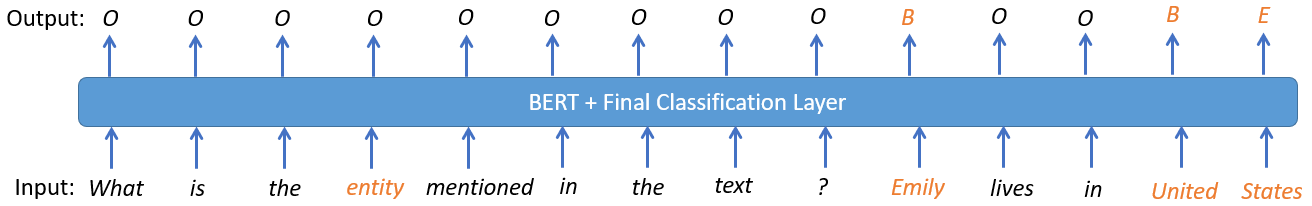
\includegraphics[width=\linewidth]{../thesis/span_detection}
    \caption{Span Detection Setup with \texttt{BIOE} scheme and \textit{What} as question word (colored tokens depict the generic entity type in question and gold entity mentions with expected output labels)}
    \label{fig:span_detection}
\end{figure}



\section{Span Classification}
\label{sec:class}
Here, we are given a sentence $\mathcal{S}$ as a $N$-length sequence of tokens, $\mathcal{S} = \langle w_1, w_2 \ldots w_N \rangle$ and a span $\langle s, e\rangle$ where $s \in [1, N]$ is the \textit{start} index, $e \in [1, N]$ is the \textit{end} index. The goal is to output a label $t$ for the span such that $t \in \mathcal{T}$, where $\mathcal{T}$ is the set of all entity types.

This is modeled as the reverse of QA model for NER described in Section \ref{sec:span}. For every gold entity mention (E.g. \textit{United States}) in a training set sentence, \textit{Emily}[\texttt{PERSON}] \textit{lives in United States}[\texttt{LOCATION}], we form a sample input, \textit{Emily lives in United States. What is United States?} The sentence is fed to a BERT model where we do sequence classification. The pooled sequence embedding returned by BERT is fed to a fully connected layer and converted to a probability distribution over possible entity types. In this example, the model is expected to assign maximum probability to \texttt{LOCATION}. Figure \ref{fig:span_classification} shows our span classification setup.

\begin{figure}[h!]
    \centering
    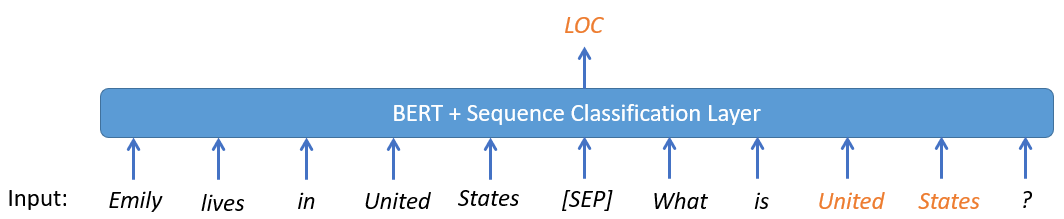
\includegraphics[width=\linewidth]{resources/span_classification}
    \caption{Span Classification Setup (colored tokens depict the entity mention in question with expected output entity label)}
    \label{fig:span_classification}
\end{figure}

- is reverse question answering setup
- is a simpler step in general compared to span detection. 
- may suffer from biases because of lots of classes and class imbalance. 
- Dice loss has been shown to be effective. So, we adopt it here as well.
- Later ablations show its effectiveness

\section{Experimental Results}
\label{sec:exp}
We have conducted extensive experiments to validate 
the effectiveness of our pipeline approach for NER tasks. 

\subsection{Data}
We validate our system using four datasets belonging to the general, biomedical and cybersecurity domains.
We use \data{OntoNotes5.0} and \data{WNUT17} for the general domain and \data{BioNLP13CG} for the biomedical domain, 
which are all publicly available.
For the cybersecurity domain, we use a private dataset, 
which contains news articles, blogs and technical reports related to malware, hacking groups and vulnerabilities.
We denote the dataset as \data{CyberThreats} in this paper.

We note that these datasets can demonstrate the effectiveness of our algorithms especially for non-word, low-resource (i.e., small number of training instances) entity types using the datasets from multiple domains and noisy text.
The datasets include not only traditional entity types with word mentions(e.g., PERSON, LOCATION) but also many entity types with non-word (Antivirus Signature) and very long mentions (e.g., URL, Software with version, etc).
Table \ref{tab:datasets_summary} shows a summary of the datasets.
\begin{table*}[h!]
\centering
\begin{small}
\begin{tabular}{ccccrrr}\toprule
 \textbf{Dataset} & \header{\#Entities} & \header{Non-Word} & \header{Low Resource} & \header{Train} & \header{Dev.} & \header{Test} \\ \toprule 
\data{BioNLP13CG} & 16 & Yes & Yes & 3,033  & 1,003 & 1,906 \\
\data{CyberThreats} & 8 & Yes & Yes & 38,721 & 6,322 & 9,837 \\
\data{OntoNotes5.0} & 18 & Yes & Yes & 115,812 & 15,680 & 12,217 \\  
\data{WNUT17} & 6 & Yes & Yes & 3,394 & 1,287 & 1,009\\
\bottomrule
\end{tabular}
\caption{Overview of the experimental datasets. \header{\#Entities} indicates the number of unique entity types.
\header{Non-Word} and \header{Low Resource} indicate if the dataset contains non-word mentions (e.g, mentions with digits and symbols) and low-resource entity types respectively.  
\header{Train}, \header{Dev.} and \header{Test} show the number of sentences in the datasets.}
\label{tab:datasets_summary}
\end{small}
\end{table*}

\yjcomment{Shall we show the class distribution for the datasets? We need to use the names of diffrent methods consistently. Let's make a name for our system instead of Span-Pipeline.}
\comment{Different domains (entity nature \& language context) / dataset sizes / No. of entities 
- BIONLP13CG: Bio dataset (using Scibert + BERT model)
- OntoNotes: General entities / newswire (using Roberta base)
- WNUT17: emerging entities from tweets (using BERT)
Also show from result analysis that span class is simpler and gives above 90\% result where as detector is the main bottleneck}

%%%%%%%%%%%%%%%%%%%%%%%%%%%%%%%%%%%%%%%%%%%%%%%%%

\subsection{Experimental Setup}
We use \deptool{transformers}\footnote{https://github.com/huggingface/transformers} library from \deptool{HuggingFace} and \deptool{pytorch} for implementation. 
For general English corpora like \data{OntoNotes5.0} and \data{WNUT17}
and the cybersecurity data, we use a pretrained BERT model (bert-base-uncased\footnote{https://huggingface.co/bert-base-uncased}). 
For the biomedical dataset (\data{BioNLP13CG}), we use SciBERT
(scibert\_scivocab\_uncased\footnote{https://github.com/allenai/scibert}), a language model for scientific text~\cite{beltagy-etal-2019-scibert}. 

Note that. in all our experiments, we only use the BERT-Base architecture, which has around 110 million trainable parameters. 
The training data is randomly shuffled and a batch size of $16$ is used with post-padding. We fixed random seed to $42$ for replication.
For BERT-based models, we set the maximum sequence length to $256$ for \data{BioNLP13CG}, \data{CyberThreats} , and \data{WNUT17} and to $512$ for \data{OntoNotes5.0}. 


We use the cross entropy loss during training unless otherwise specified. 
The development set evaluation takes place at steps of 0.5 training epochs. We train the models for $300$ epochs at learning rate $10^{-5}$ unless otherwise specified.
The BERT-based models output entity labels for each sub-token (as per WordPiece tokenization) of an existing token in the dataset. 
We take the label of the first sub-token as the label for the corresponding token for the evaluations.
We use Nvidia GeForce GTX 1080 and Nvidia Tesla V100 GPUs for model training and evaluation.

%%%%%%%%%%%%%%%%%%%%%%%%%%%%%%%%%%%%%%%%%%%%%%%%%

\subsection{Baseline Systems}
\yjcomment{Jatin -- please update this section}


We present this comparison since QA model serves as the primary backbone of our span-based approach. 
All models here use BIOE tagging scheme.
For span detection, we use \textit{Extract important entity spans from the following text} as the question irrespective of the entity types.
For span classification, we use \textit{What is $<mention>$} where $<mention>$ is the string value for an extracted span by the span detection model.  

\if false  
\texttt{BERT}: Proposed by \cite{devlin2018bert}, BERT is a bidirectional encoder transformer\cite{vaswani2017attention}. It applies WordPiece\cite{wu2016google} tokenization on input sentence which is then passed through several encoder layers with multiple attention heads capturing sentence semantics and inter-token relationships well. The model outputs contextualized embeddings for each sub-token in the sentence. We take the last hidden layer outputs from BERT model and pass it to a fully connected layer. The outputs are converted to a probability distribution over labels space. Model parameters are initialized from a pretrained model and fine-tuned on our NER task.


\texttt{BERT-Freeze}: To understand how much semantic information is already captured in a pretrained BERT model, we use the exact same architecture as \texttt{BERT} model above but freeze the BERT model parameters. So, the only trainable parameters remain from the fully connected layer. For this setting, we use learning rate as $0.005$.

\texttt{CNN-LSTM-CRF}: \comment{better to include this as a baseline since it is very widely used}
\fi

\subsection{Performance Comparison}
We compare the performances of our system, the baseline systems and the best reported 
state-of-the-art (SOTA) tools. 
All of our models' results were measured on the test sets using the model checkpoint corresponding to the best Micro F1-score on the development sets. 
Table~\ref{tab:res_span} shows the comparison results based on the mention-level Micro F1 scores on the test sets (i.e., only the exact matches are considered correct).
\begin{table*}[h!]
\centering
\begin{small}
\begin{tabular}{ccccc}\toprule
 \textbf{Model} & \texttt{BioNLP13CG} & \texttt{CyberThreats} & \texttt{OntoNotes} & \texttt{WNUT17} \\ \toprule 
BERT-QA & 86.69 & \textcolor{blue}{ongoing(y1)} & \textcolor{blue}{ongoing(j)}  & 44.60 \\
BERT-Span-Pipeline-Vanilla     & 86.69 & \textcolor{red}{todo} & 90.12 & 55.36  \\
BERT-Span-Pipeline     & 86.70 & \textcolor{red}{todo} & 90.31 & 56.30  \\
Reported SOTA & 85.56(thesis see) & N/A & 92.07(MRC-Dice) & 60.45(CL-KL)  \\
\bottomrule
\end{tabular}
\caption{Comparison of the NER results on the four datasets. The numbers indicate the mention-level Micro F1 scores. 
\yjcomment{can you find the results of SOTA without any external data or additional pretraining? I consider MRC-Dice also using additional info. as they added several synonyms/hyponyms in query.   we can put SOTA without external data and with external data in separate rows if you like. We point out that our system does not rely on external knowledge which is usually unavailable for domain-specific data and needs less computing resources than MRC}}
\label{tab:main}
\end{small}
\end{table*}

\paragraph{Feature Analysis}
To investigate the effectiveness of the character sequence and pattern embeddings,
we performed the span detection tasks with and without the character and pattern features.
In Table~\ref{tab:det_ablation}, we report the mention-level precision (P), recall (R) and F1 scores
by the two models. 
As we can from the results, adding pattern and character features improve the precision while
maintaining similar recall levels.
\begin{table*}[h!]
\centering
\begin{small}
\begin{tabular}{ccccccccccccc}\toprule
 \multirow{2}{*}{\textbf{Model}} & \multicolumn{3}{c}{\data{BioNLP13CG}} & \multicolumn{3}{c}{\data{CyberThreats}} & \multicolumn{3}{c}{\data{OntoNotes5.0}} & \multicolumn{3}{c}{\data{WNUT17}} \\ \cmidrule{2-12} 
 & P & R & F1 & P & R & F1 & P & R & F1 & P & R & F1 \\ \midrule
Char-Pattern & 91.43 & 90.70 & 91.06 & & & 78.63 \textcolor{blue}{ongoing(y4)}& & & 92.50 & & & 55.21  \\
No Char-Pattern& & & 90.67 &79.65 & 77.77 & 78.70 & & & 92.37 & 72.63 & 44.06 &54.85  \\
\bottomrule
\end{tabular}
\caption{Performance comparison of span detection with and without character and pattern embeddings}
\label{tab:det_ablation}
\end{small}
\end{table*}


\paragraph{Loss Function}
A recent study has shown that using dice coefficient as the loss function was more beneficial than 
the cross entropy loss for NLP tasks with imbalanced data~\cite{li2019dice}. 
Inspired by this work, we trained our span classification model, which has the data imbalance problem,
using both cross entropy loss and dice loss.
Our experiments also confirm that the dice loss provides a small improvement over the cross entropy loss 
as shown in Table~\ref{tab:class_ablation}.
\begin{table*}[h!]
\centering
\begin{small}
\begin{tabular}{ccccc}\toprule
 \textbf{Model} & \texttt{BioNLP13CG} & \texttt{CyberThreats} & \texttt{OntoNotes} & \texttt{WNUT17} \\ \toprule 
Span-Classification-Dice & 94.27 & 87.84 &  96.74 & 73.40  \\
Span-Class-CE     & 94.04 & 87.58 & 96.50 & 73.31  \\
\bottomrule
\end{tabular}
\caption{Span Classification Results with different loss functions}
\label{tab:class_ablation}
\end{small}
\end{table*}

\paragraph{Training Time}
As discussed in Section~\ref{sec:method}, our pipeline approach applying span detection  and span classification separately is more efficient than combined models.
To validate the assertion, we measured the training times of our pipeline system
and the baseline BERT-QA, which uses exactly the same features and underlying architecture but performs span detection and classification in one unified model.
All experiments were done using two V100 GPUs with 16G memory on each GPU. 
The results confirm that the pipeline approach is much more efficient,
and, the efficiency improvement grows as the size of training data and 
the number of entity types grow.
\begin{table*}[h!]
\centering
\begin{small}
\begin{tabular}{ccccc}\toprule
 \textbf{Model} & \texttt{BioNLP13CG} & \texttt{CyberThreats(10\%)} & \texttt{OntoNotes(10\%)} & \texttt{WNUT17} \\ \toprule 
BERT-QA                & 1,372.8 & 877.1 &  7,381.8   & 568.2\\
Span-Pipeline     & 241.2 (106.3/134.9) & 145.53 (113.7/31.9) & 300.8 (185.5/115.3)  & 122.9 (98.9/24.0)\\
\bottomrule
\end{tabular}
\caption{Comparison of the training time between our method and a non-pipeline QA-based NER method. 
    The training time is reported in seconds per training epoch. The numbers in the parentheses denote the training times for span detection and span classification respectively. }
\label{tab:train_time_ablation}
\end{small}
\end{table*}

\begin{table*}[h!]
\centering
\begin{small}
\begin{tabular}{cccccc}\toprule
      &  \textbf{} & BioNLP13CG & JNLPBA & CoNLL2003 & OntoNotes5.0\\\toprule
\multirow{3}{*}{Baseline} & \texttt{BERT-Freeze} &  75.42 & 55.93 & 82.79 & 67.35 \\
                          & \texttt{BERT} & 85.99 & 74.35 & 91.36 & 83.39 \\ 
                          & \texttt{BERT-QA} & \textbf{86.45} & 74.81 & 91.17 & \\\midrule
\multirow{3}{*}{OurModel} &        \texttt{Span Detection} & 90.12 & 78.35 & 95.23 & \\
        & \texttt{Span Classification} & 94.06 & 95.08 & 94.50 & \\
        & \texttt{Pipeline} & 85.89 & \textbf{75.01} & \textbf{91.64} & \\ \bottomrule
\end{tabular}
\caption{The classificaiton results of our system and the state of the art method over 4 benchmark datasets. 
     The numbers reprent the Micro-F1 in \% on the test datasets.}
    \label{tab:res_span}
\end{small}
\end{table*}

%\comment{need more results and some plots}

\if false
Next, we deep dive into the \texttt{BioNLP13CG} dataset which has $16$ entity types including several high and low-resource types. We compare the model performance at the entity type level for our 3 major NER approaches: sequence labeling, question answering and span-based pipeline. We compare our best performing model variants through entity-level and macro-averaged F1-scores. Let $\mathcal{T}$ be the set of all entity types and F1$_t$ be the F1-score for individual entity type $t \in \mathcal{T}$. Then, Macro-averaged F1-Score is defined in Equation \ref{eq:macro_f1} as:
\begin{equation}
\label{eq:macro_f1}
    \text{Macro-F1} = \frac{1}{\mathcal{\vert\mathcal{T}\vert}}\,\sum_{t\,\in\,\mathcal{T}}{\text{F1}_t}
\end{equation}
We present the comparison among the following models:
\begin{itemize}
    \item \texttt{Dice Loss}: Sequence labeling NER approach over BERT model with \texttt{BIO} tagging scheme and dice loss instead of cross entropy.

    \item \texttt{Special Symbol}: Sequence labeling NER approach over BERT with \texttt{BIO} tagging scheme and additional one-hot input feature to capture if a token is a special symbol like \textit{hyphen}, or \textit{parenthesis}.

    \item \texttt{BERT-QA (Where)}: Question answering NER approach with \texttt{BIOE} tagging scheme and \textit{Where} as the question word.

    \item \texttt{Span Based}: Pipelined approach which uses the QA setup with \texttt{BIOE} tagging scheme and \textit{What} as question word for span detection and QA-based sequence classification for span classification.
\end{itemize}

\begin{figure}
    \centering
    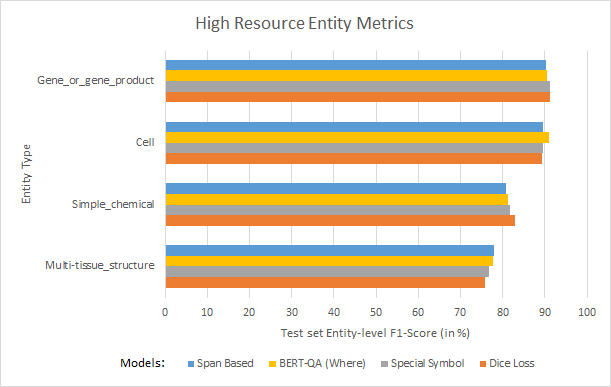
\includegraphics[scale=0.5]{../thesis/high_resource_entity_metrics}
    \caption{Test set Entity-level F1 scores for high resource entities in \texttt{BioNLP13CG} dataset}
    \label{fig:high_resource_entity_metrics}
\end{figure}

\begin{figure}
    \centering
    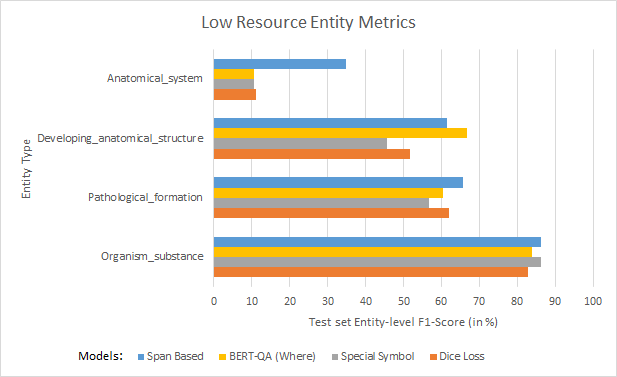
\includegraphics[scale=0.5]{../thesis/low_resource_entity_metrics}
    \caption{Test set Entity-level F1 scores for low resource entities in \texttt{BioNLP13CG} dataset}
    \label{fig:low_resource_entity_metrics}
\end{figure}

\fi


\section{Related Work}
\label{sec:related}
\textbf{CrossWeigh}~\cite{WangSLLLH19} considers a method to handle label mistakes during NER model training.

It partitions the training data into several folds and train independent NER mod- els to identify potential mistakes in each fold and then adjusts the weights of training data accordingly to train the final NER model.
The technique is similar to k-fold cross validation with \textit{entity disjoint filtering}.
(1) split the training data into k folds.
(2) collect all entity mentions (only mentions and not entity types)  in a fold (i) (called test entities)
(3) remove all sentences that contain the test entities from the training data for the i-th fold 
(4) train k models and test them
(5) find sentences that contain at least one mis-classification
(6) compute confidence for each sentence indicating the likelihood the sentence containing  mislabels.
However, this method works well when the initial model has high confidence of being accurate (>90\% general accuracy).
·        Data Setting: CoNLL2003 English NER
·        Performance: Leads to ~0.5\% improvements due to label corrections

\textbf{Contextual string embeddings}~\cite{akbik-etal-2018-contextual} models words as sequences of characters contextualized by their surrounding text.
It passes  sentences as sequences of characters into a character-level language model to form word-level embeddings.
It leverages pre-trained character-level language models from which they extract hidden states at the beginning and end character positions of each word to produce embeddings for words.
The embedding of a word is the concatenation of the hidden states of fLM and bLM of its character sequences.
This results in different embeddings for the same word when it is used in different contexts and has shown a significant improvement for sequence labeling tasks such as NER and Chunking.
The main advantages are: (1) pre-train on large unlabeled corpora, (2) capture word meaning in context and therefore produce different embeddings for polysemous words depending on their usage, and (3) model words and context fundamentally as sequences of characters, to both better handle rare and misspelled words as well as model subword structures such as prefixes and endings.
For NER, the best performance was achieved by Contextual string embeddings + pretrained word embeddings + task-trained character features in a hierarchical BiLSTM-CRF architecture 
closely followed by Contextual string embeddings + pretrained word embeddings (Glove) indicating that task-trained character features are subsumed by character embeddings.


\textbf{W-NUT (Workshop on Noisy User-generated Text)} uses training data from Twitter and development/testing data from Reddit, YouTube, Twitter and StackOverflow data.
Entity types include Person, Location, Corporation, Product, Creative-work, Group.
The best F1 is currently 49.59 by Akbik et al.~\cite{akbik-etal-2019-pooled}.

\textbf{Pooled contextualized embeddings}~\cite{akbik-etal-2019-pooled} address the drawback of the contextualized character-level models which suffer 
from an inherent weakness when encountering ``rare words in an underspecified context``.
However, they assume that these rare entities are normally only used in underspecified contexts \textit{if they are expected to be known to the reader}. 
That is, they are either more clearly introduced in an earlier sentence, or part of general in-domain knowledge.

They aggregate the contextualized string embeddings of each unique string 
 and thus produces \textit{evolving word representations} that change over time as more instances of the same word appear. 

For each word in a sentence, the word representation is a concatenation of its contextualized word embedding generated by~\cite{akbik-etal-2018-contextual} and a pooling of
all embeddings of the word seen so far.

\textbf{A Little Annotation does a Lot of Good: A Study in Bootstrapping Low-resource Named Entity Recognizers}~\cite{ChaudharyXSNC19}
proposes a bootstrapping approach for NER for low-resourced languages.
It applies a cross-lingual transfer learning to project annotations from English data to the target language (with word embeddings of both source and target languages, a bilingual dictionary and labeled data for the source language), then apply activie learning
and bootstrapping of the model.
To reduce human labeling efforts, they label only subspans of sentences where named entities most likely appear and apply partial CRFs to learn from the annotated subspans.
(see Algorithm 1 for the potential entity span detection method).

·        Idea: Transfer Learning then Bootstrapping (using manual active learning)
·        Data Setting: CoNLL English, Hindi, Spanish, Indonesian NER
·        Model: CNN-BiLSTM-CRF (for NER). Initially train Bilingual word embeddings then transfer knowledge to label unlabeled low-resource corpus. Train CNN-BiLSTM-CRF model for NER on it. Use marginal prob. to get entity spans with high uncertainty for human labeling. Augment to corpus and retrain NER model iteratively. Use partial-CRF for NER, since, sentences are partially gold annotated, for other parts of the sentence, the loss should not affect the model (since, those parts are not yet labelled)
·        Performance: +9 points in F1 (around) than other active learning or transfer learning techniques.

1. Dual Adversarial Neural Transfer for Low-Resource Named Entity Recognition~\cite{ZhouZJZFGK19}
·        Idea: adversarial modifications can help in knowledge transfer in low-resource settings
·        Data Setting: Cross-Lang (Eng to Spanish/Dutch), Cross-Domain (CoNLL English to Tweets English) knowledge transfer
·        Model: CNN-BiLSTM-CRF arch. with adversarial perturbations (introduced for robust training in low-resource setting)
·        GRAD loss (for shared parameters): basically linear transformation over self-attention then log likelihood of that.
o   Not sure how it would work without softmax? (1 - r) term: how does it work?
o   How is the linear transformation params decided?
·        Overall loss: label loss (source and target) (CRF) + GRAD loss
·        Performance: Comparable performance in high-resource and better performance in low-resource setting
 
 
 
4.      Improving Distantly-supervised Entity Typing with Compact Latent Space Clustering~\cite{PengXZFH19}
·        Idea: Distant supervision leads to noisy training data. Existing denoising methods rely on partial label loss objective which leads to confirmation bias (as it corrects data based on its own objective function). So, try to cluster similar entity mentions together instead.
·        Model: LSTM based for entity typing, minimizing KL divergence between predicted and actual entity labels
·        Compute embedding representation before passing to final classifier and make distance-graph out of them. Then, do label propagation on graph for clustering and revise embedding representation through a loss.
·        Data Setting: OntoNotes, BBN (news/wall street journal based)
·        Performance:  Compared to partial label loss, partial label embedding, joint representation of entity mentions and label types etc. approaches. 1-2\% F1 improvement.
 
5.      Exploiting Structure in Representation of Named Entities using Active Learning~\cite{BhutaniQ0JHV18}
·        Idea: Implicit structure in named entities (which is very task-dependent)
·        Model: Active Learning where user supplies some structures, model proposes more which the user can correct/reward. Edit distance among structures calculated. Rule generation based on pattern matches in corpus.
·        Data Setting: Person/Company mentions etc. from ACE
·        Performance: 3\% F1 better on company, similar on Person (than CRF-based)


Pattern (Regex) Understanding with Deep Learning:
1.      Deep Learning for Regex (Blog): Learning to identify alpha-numeric Product ID from text sentences (deep char-level embeddings learning implicit regular expression formats) (data/code not available)
 
2.      Marrying Up Regular Expressions with Neural Networks: A Case Study for Spoken Language Understanding (ACL'18): Matching regexes in sentences and using the matched words for manipulating attention weights etc. in a standard BiLSTM framework for sentence classification (intent detection) and sequence labelling (slot filing) tasks. Dataset: ATIS + manually created regexes (data available here)
 
3.      DeepRegex: Generating Regular Expression from Natural Language Description (EMNLP'16): Uses LSTM-based seq-2-seq arch., dataset(NX-RX, semi-manually created) has 10,000 regexes with single sentence descriptions. Code based on Pytorch and Lua (GitHub) (some positive and negative generated samples described here)
 
4.      Understanding Regex using Deep Learning (Blog): generating natural language description of regexes (opposite of DeepRegex). Used same data and model architecture. (data/code)
 
5.      Generating Regular Expressions from Natural Language Specifications: Are We There Yet? (AAAI'18): Basically, evaluates DeepRegex (described above) on NX-RX dataset and a real-world RegexLib dataset (not available). Says, NX-RX dataset is synthetic and in real-world, this system, DeepRegex, still does not perform too well.
a.      Proposes that large real-world corpus should be made for better training
b.      Model should use positive and negative examples of regex match, apart from the seq-2-seq arch. for better regex interpretation
 
6.      Inference of Regular Expressions for Text Extraction from Examples (TKDE'16): Automatically generating regular expressions from examples/given matches. (uses genetic algorithms) (slides, code, demo)
 
Numeral Understanding with Deep Learning:
1.      Numerical Polysemy (Challenge with numbers/alpha-numerics): Number '12' can have diverse meanings in different sentences based on context! It can be a month, date, age, size of plot etc. So, a single embedding for number 12 is not a good idea. Contextual embeddings would be better! Similar thing happens with words too, like, 'bank' but has less diverse range of meanings.
 
2.      Numeracy-600K: Learning Numeracy for Detecting Exaggerated Information in Market Comments (ACL'19): Prepared data from market comments on Reuters. Predict number range (among 8 classes) for filling a blank related to the market comment. Found Bi-GRU framework working best. (Dataset)
 
3.      Do NLP models know numbers? (ACL'19): Pretty good analysis showing that Word2Vec, GloVe, char-CNN embeddings, ELMo, BERT all have some good sense of number representation. Tested on numerical Q/A dataset (DROP - made by AllenNLP). Found char-level embeddings are able to represent numbers better than word embeddings. CNNs arch. are able represent numbers better. ELMo gives better performance than BERT.
 
4.      Learning Numeral Embeddings(submitted to ICLR'20): Learning number embeddings by sampling some representative numbers out, embedding them, then for any other number, do soft clustering by learning a GMM over those representative number's embeddings.



\section{Conclusion}
Taking inspiration from the QA setup, we proposed the span detection and classification pipeline which uses a reverse question formulation. We also proposed to convert from a sparse character space to a dense pattern space through which we can learn meaningful intrinsic character patterns in alphanumeric and pattern-oriented entities. We demonstrated the effectiveness of our proposed domain-agnostic techniques on multiple datasets in general English and biomedical domains. 
%We also presented a study depicting that trivial concatenation of external semantic vectors with BERT outputs may not train the model effectively at lower learning rates.

Our span-based setup opens up prospects for more intuitive and creative ways of approaching the NER problem. However, the pipelined nature of the approach currently serves as a bottleneck. It may be worthwhile to think of some ensemble-based approach where we train individual BERT models on some sub-problems and each of those models contributed its part to solve the overall NER problem in a majority-voting setup.

%Our study on training effectiveness reveals that feeding additional external semantics while fine-tuning the BERT model is non-trivial. This again motivates future research on designing feature fusion techniques which are effective with a BERT (transformer-like) architecture.

From the qualitative analysis of the various approaches, we observe that boundary detection serves as a primary issue in NER. To alleviate this problem, we explicitly model word types and special symbols. However, there is still a wide margin to cover. We encourage the research community to design architectures or new training objectives tailor-made to handle mention boundaries effectively. 


%\section*{Acknowledgements}

% Entries for the entire Anthology, followed by custom entries
\bibliographystyle{styles/acl_natbib}
\bibliography{thesisrefs.bib}
%\bibliography{anthology,custom}

%\appendix

%\section{Example Appendix}
%\label{sec:appendix}


\end{document}
